\documentclass[UTF8]{ctexart}

\usepackage{amsmath}
\usepackage{listings}
\usepackage{graphicx}   % used to insert graphs

\title{Computer Networking Homework3}
\author{PB22111620 Ai Chang}

\begin{document}
\begin{sloppypar}
\maketitle

\subsection*{1}

C. TCP 识别的是字节流,所以不可能是91. TCP 采用累积确认,且并未规定是否可以乱序接收。
若 TCP 可以乱序接收: TCP 在接收题述分段前可能已经接受了序号为 190 的数据,故确认号可
以不是 190. 若 TCP 接收序号为 90 的数据前未接收前面的数据,如序号为 40, 包含 50 个
字节的数据,其确认号就会小于 90. 若 TCP 接收序号为 90 的数据前接受了后续的数据,如序
号为 190, 包含 100 个字节的数据,则确认号是 290, 故可以大于 190. 综上,答案是 c

\subsection*{2}

对二者求和得到 0001\_1011 且有进位, 回卷得到 0001\_1100, 故校验和为 1110\_0011。
eg: 两个数最高位均出错, 故接收方得到的数为 1110\_0010, 0011\_1001, 求和、回卷
得到的值为 0001\_1100, 与校验和相加后为 1111\_1111, 故两个数各有一个 bit 出错
时, 校验和无法检验差错

\subsection*{3}
    此题中 cwnd, ssthresh 的单位均为 MSS, 回答中省略
    \subsubsection*{(a)}
        拥塞控制算法是 Reno, 因为在时间 22-23 时, cwnd 从 24变为 15,
        即 $cwnd= cwnd/2 + 3$ 而不是直接降为 1
    \subsubsection*{(b)}
        根据 cwnd 从指数增长变为线性增长的节点判断, 初始 ssthresh = 32
    \subsubsection*{(c)}
        cwnd 在时间 10 直接降为 1, 可知该时刻发生了超时。
        时间 11, ssthresh = 18, cwnd = 1
    \subsubsection*{(d)}
        cwnd 在时间 22 从 24 降为 15, 可知该时刻发送端收到三个冗余 ACK,
        出现了丢包。时间 23, ssthresh = 12, cwnd = 15
    \subsubsection*{(e)}
        cwnd 在时间 36 直接降为 1, 可知该时刻出现超时。
        时间 37, ssthresh = 14, cwnd = 1
    \subsubsection*{(f)}
        由 1 + 2 + 4 + 8 + 16 = 31, 31 + 32 = 63, 可知第 32-63 个分段
        均为时间 5-6 中发送的,所以第 50 个分段是在时间 5-6 中发送的
    \subsubsection*{(g)}
        根据慢启动阶段 cwnd 呈指数增长来判断, 1-6, 11-15, 37-41 TCP 均为慢启动状态

\subsection*{4}
    \subsubsection*{Graph 1:}
        (1) 75 (2) 75 (3) 80
    \subsubsection*{Graph 2:}
        (1) 40 (3) 40 (3) 40 (4) 70
    \subsubsection*{Graph 3:}
        (1) 30 (2) 30 (3) 50

\subsection*{5}
    \subsubsection*{(a)}
        依题,设 cwnd 最大是 n 个 TCP 分段,则发送速率为
        $$\frac{n \times 1500 byte}{150ms} = 80n kbps$$
        由$$80n kbps < 10 Mbps$$得$$n < 125$$
        故发送端的拥塞窗口最大可以是 125 个 TCP 分段;
        
        若因为超时发现丢包, cwnd 大小为 1 个 TCP 分段。
        若发现三个冗余 ACK 发现丢包, cwnd 大小为 $n = 125/2 + 3 \approx 65$
         个 TCP 分段.
        
        发送端平均吞吐率为$$throughput = \frac{3}{4} * \frac{W}{RTT}= 7.5 Mbps$$
    \subsubsection*{(b)}
        \begin{enumerate}
            \item 若发送端通过定时器超时发现丢包, cwnd 降为 1, ssthresh 变为 62,
                先进入慢启动阶段,经过 6RTT 的时间 cwnd 倍增至 62, 然后进入拥塞避免
                模式,总时间为 \[T = (6 + 63) \times RTT = 10.35s\]
            \item 若发送端通过收到三个冗余 ACK 发现丢包, cwnd 降为 62, 进入拥塞避免
                模式, 每个 RTT 增加 1MSS, 共需时间 \[T = 63 \times RTT = 9.45s\]

                
        \end{enumerate}

\subsection*{6}
    \begin{enumerate}
        \item 若采用停等方式传输数据,链路的利用率为$$U_{sender} =
            \frac{L/R}{RTT + L/R} = 0.553\%$$
        \item 若采用流水线方式,由$$\frac{n \times L/R}{RTT
        + n \times L/R} \geq 50\%$$得$$n \geq 187.5$$
        故$$n_{min} = 188$$
    \end{enumerate}

\subsection*{7}
    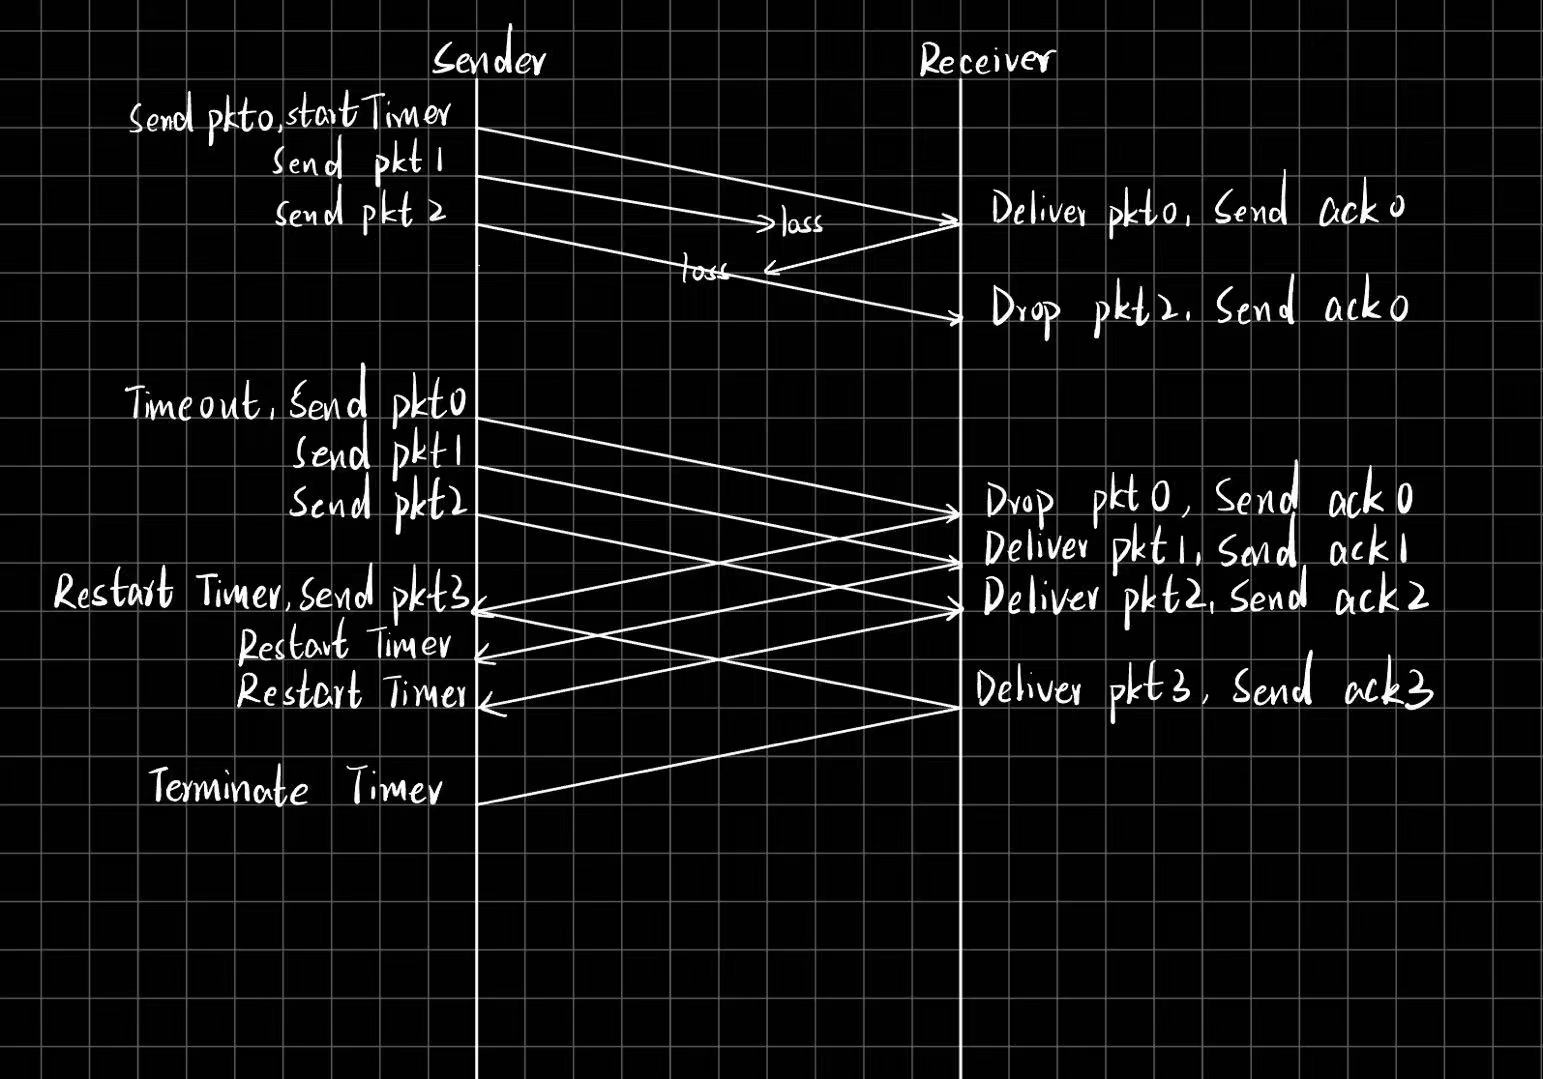
\includegraphics[width = .8\textwidth]{Q7_Answer.jpg}

\subsection*{8}
    \subsubsection*{(1)}
        因为从 A 开始发送数据算起, cwnd 开始呈指数增长,其值依次
        为$1MSS, 2MSS, 4MSS, 8MSS$,故在该过程中 A 总共发送了 15KB 的数据
    \subsubsection*{(2)}
        因为在整个发送过程中没有发生丢包,所以 cwnd 在达到 8MSS 后进入阻塞避免阶段,
        其值依次为`9MSS, 10MSS, 11MSS', 而$$(15 + 9 + 10)KB = 34KB < 40KB <
        45KB = (34 + 11)KB$$故从 A 开始发送数据到 B 收到全部数据经过了七个 RTT,
        即$$T = 7 \times RTT = 70ms$$
    \subsubsection*{(3)}
        从 A 开始发送数据到 cwnd == 10KB 的过程时间为 5RTT 即 50ms, 此时发生超时
        事件意味着 A 还未收到来自 B 的任何分段. A 将 cwnd 设为 1, ssthresh 设
        为 5MSS 并重新发送所有分组,之后 cwnd 的值依次为 1MSS, 2MSS, 4MSS, 5MSS,
        6MSS, 7MSS, 8MSS, 9MSS, \dots. 与(2)类似的,可以得出在 cwnd == 9MSS
        之前 B 收到全部数据,总时间为$$T = 50ms + 7 \times RTT = 120ms$$

\end{sloppypar}
\end{document}